\def\year{2022}\relax
%File: formatting-instructions-latex-2022.tex
%release 2022.1
\documentclass[letterpaper]{article} % DO NOT CHANGE THIS
\usepackage{graphicx}
\graphicspath{ {../../data/} } %might need to change this if you're compiling on overleaf!
\usepackage{aaai22}  % DO NOT CHANGE THIS
\usepackage{times}  % DO NOT CHANGE THIS
\usepackage{helvet}  % DO NOT CHANGE THIS
\usepackage{courier}  % DO NOT CHANGE THIS
\usepackage[hyphens]{url}  % DO NOT CHANGE THIS
\usepackage{graphicx} % DO NOT CHANGE THIS
\urlstyle{rm} % DO NOT CHANGE THIS
\def\UrlFont{\rm}  % DO NOT CHANGE THIS
\usepackage{natbib}  % DO NOT CHANGE THIS AND DO NOT ADD ANY OPTIONS TO IT
\usepackage{caption} % DO NOT CHANGE THIS AND DO NOT ADD ANY OPTIONS TO IT
\DeclareCaptionStyle{ruled}{labelfont=normalfont,labelsep=colon,strut=off} % DO NOT CHANGE THIS
\frenchspacing  % DO NOT CHANGE THIS
\setlength{\pdfpagewidth}{8.5in}  % DO NOT CHANGE THIS
\setlength{\pdfpageheight}{11in}  % DO NOT CHANGE THIS
\usepackage{multirow}
\usepackage{array}
\newcolumntype{M}[1]{>{\centering\arraybackslash}m{#1}}
\setlength{\extrarowheight}{4pt}
\usepackage[colorinlistoftodos]{todonotes}
\usepackage[colorlinks=true, allcolors=blue]{hyperref}
%
% These are recommended to typeset algorithms but not required. See the subsubsection on algorithms. Remove them if you don't have algorithms in your paper.
\usepackage{algorithm}
\usepackage{algorithmic}

%
% These are are recommended to typeset listings but not required. See the subsubsection on listing. Remove this block if you don't have listings in your paper.
\usepackage{newfloat}
\usepackage{listings}
\setlength{\parskip}{1em}
\lstset{%
	basicstyle={\footnotesize\ttfamily},% footnotesize acceptable for monospace
	numbers=left,numberstyle=\footnotesize,xleftmargin=2em,% show line numbers, remove this entire line if you don't want the numbers.
	aboveskip=0pt,belowskip=0pt,%
	showstringspaces=false,tabsize=2,breaklines=true}
\floatstyle{ruled}
\newfloat{listing}{tb}{lst}{}
\floatname{listing}{Listing}
%
%\nocopyright
%
% PDF Info Is REQUIRED.
% For /Title, write your title in Mixed Case.
% Don't use accents or commands. Retain the parentheses.
% For /Author, add all authors within the parentheses,
% separated by commas. No accents, special characters
% or commands are allowed.
% Keep the /TemplateVersion tag as is
\pdfinfo{
/Title (AAAI Press Formatting Instructions for Authors Using LaTeX -- A Guide)
/Author (AAAI Press Staff, Pater Patel Schneider, Sunil Issar, J. Scott Penberthy, George Ferguson, Hans Guesgen, Francisco Cruz, Marc Pujol-Gonzalez)
/TemplateVersion (2022.1)
}

\usepackage{blindtext}

% DISALLOWED PACKAGES
% \usepackage{authblk} -- This package is specifically forbidden
% \usepackage{balance} -- This package is specifically forbidden
% \usepackage{color (if used in text)
% \usepackage{CJK} -- This package is specifically forbidden
% \usepackage{float} -- This package is specifically forbidden
% \usepackage{flushend} -- This package is specifically forbidden
% \usepackage{fontenc} -- This package is specifically forbidden
% \usepackage{fullpage} -- This package is specifically forbidden
% \usepackage{geometry} -- This package is specifically forbidden
% \usepackage{grffile} -- This package is specifically forbidden
% \usepackage{hyperref} -- This package is specifically forbidden
% \usepackage{navigator} -- This package is specifically forbidden
% (or any other package that embeds links such as navigator or hyperref)
% \indentfirst} -- This package is specifically forbidden
% \layout} -- This package is specifically forbidden
% \multicol} -- This package is specifically forbidden
% \nameref} -- This package is specifically forbidden
% \usepackage{savetrees} -- This package is specifically forbidden
% \usepackage{setspace} -- This package is specifically forbidden
% \usepackage{stfloats} -- This package is specifically forbidden
% \usepackage{tabu} -- This package is specifically forbidden
% \usepackage{titlesec} -- This package is specifically forbidden
% \usepackage{tocbibind} -- This package is specifically forbidden
% \usepackage{ulem} -- This package is specifically forbidden
% \usepackage{wrapfig} -- This package is specifically forbidden
% DISALLOWED COMMANDS
% \nocopyright -- Your paper will not be published if you use this command
% \addtolength -- This command may not be used
% \balance -- This command may not be used
% \baselinestretch -- Your paper will not be published if you use this command
% \clearpage -- No page breaks of any kind may be used for the final version of your paper
% \columnsep -- This command may not be used
% \newpage -- No page breaks of any kind may be used for the final version of your paper
% \pagebreak -- No page breaks of any kind may be used for the final version of your paperr
% \pagestyle -- This command may not be used
% \tiny -- This is not an acceptable font size.
% \vspace{- -- No negative value may be used in proximity of a caption, figure, table, section, subsection, subsubsection, or reference
% \vskip{- -- No negative value may be used to alter spacing above or below a caption, figure, table, section, subsection, subsubsection, or reference

\setcounter{secnumdepth}{0} %May be changed to 1 or 2 if section numbers are desired.

% The file aaai22.sty is the style file for AAAI Press
% proceedings, working notes, and technical reports.
%

% Title

% Your title must be in mixed case, not sentence case.
% That means all verbs (including short verbs like be, is, using,and go),
% nouns, adverbs, adjectives should be capitalized, including both words in hyphenated terms, while
% articles, conjunctions, and prepositions are lower case unless they
% directly follow a colon or long dash
\title{COVID-19 on Twitter: Heated Discussions}
\author{  \\Antoine Bonnet, \\
antoine.bonnet@mail.mcgill.ca,
\\[3ex]
Rahul Kumar,\\
rahul.kumar2@mail.mcgill.ca, 
\\[3ex]
Fabrizzio Sabelli,\\
fabrizzio.sabelli@mail.mcgill.ca\vspace{0.5cm} }

% REMOVE THIS: bibentry
% This is only needed to show inline citations in the guidelines document. You should not need it and can safely delete it.
%\usepackage{bibentry}
% END REMOVE bibentry

\begin{document}

% The report must be between 5 and 7 pages in length, not including references. Figures are encouraged – but should be used to maximum effect (fluffy or otherwise unnecessary images that do not make strong contributions to the report will lead to point deductions).


\maketitle

\section{Introduction}

% 0.5 page. General overview and key findings

% Do this last

% 1. Goal

The objective of this project was to analyze COVID-19 related Twitter discussions to uncover general trends in sentiment towards sanitary measures and vaccination in English-speaking countries. 

% 2. Methods used for attaining goal

To attain this goal, 1000 Tweets linked with the pandemic were collected from Twitter using appropriate filters. By open coding, 7 topics of discussions were identified in relation to the COVID-19 pandemic. Each Tweet was then annotated manually to identify its most salient topic, and its position towards the sanitary measures imposed by the government for the pandemic (including quarantine and vaccination) was evaluated. 

After the annotation process, textual analysis was performed on Tweets grouped by each category. The most recurrent words pertaining to each topic were identified using the textual-frequency inverse-document-frequency (TF-IDF) metric. Other statistics pertaining to the distribution of sentiment across topics were also calculated. 

% 3. Results and findings

We found that most tweets were factual in nature and were providing
statistics and/or information around the pandemic. The most controversial topic
by far was tweets involving discussion on vaccinations and vaccine regulations.
Overall, there is a positive response by users towards measures taken to combat the pandemic.

\section{Data}

% 0.5 page. Describe your dataset. This should include statistics relevant to the project – the number of tweets you originally started with, the keywords used to collect tweets, and any design decisions you had to make around the filtering of this content.

% Was the dataset prepared correctly? Did it have baseline characteristics that would allow this study to deliver meaningful insights?

% Keywords used to collect tweets

A list of 27 keywords related to COVID-19 was constructed in order to collect Tweets containing at least one keyword. This list contains multiple derivations of the COVID-19 name, principal vaccine manufacturers, as well as words related to the pandemic and sanitary measures: 

\vspace{0.1cm}

\begin{table}[htb]
\caption{COVID-19 related keywords used for Twitter data collection.}
  \centering
\begin{tabular}{|M{2cm}|M{2cm}|M{2.8cm}| }
 \hline 
 COVID & immunization & injection\\
 COVID-19 & symptoms & dose\\
 COVID19 & symptomatic & AstraZeneca\\
 coronavirus & epidemic & BioNTech\\
 pandemic & vax & Johnson \& Johnson\\
 quarantine & vaxx & Moderna\\
 screening & vaxxed & Pfizer\\
 distancing & vaccine & Sanofi\\
 immunity & vaccination & Sinopharm\\
 \hline
\end{tabular}
\end{table}

\vspace{0.1cm}


From these keywords, 1000 different Tweets were collected on December 6th, 2021. After scraping, the dataset was reviewed informally and we realized that a few Tweets (approximately 4\%) had been incorrectly picked up by a keyword and were unrelated to the COVID-19 pandemic. We identified these faulty data points, excluded from our analysis and collected new Tweets so as to obtain a dataset of 1000 relevant Tweets in our dataset. The original tweets and new tweets were also collected during a 3 day window. Following the scraping, we annotated the dataset according to techniques we will discuss later. Each tweet has a sentiment annotation and topic annotation. 

\section{Methods}

% 0.5 page. Explanation and justification for what you did. Focus on the design decisions you made NOT listed in this document that impacted your results.

Our textual analysis is based on the semantic meaning of words used in the Tweets. We therefore filtered out common English words (also called stopwords) from our database by removing all words in the list made available by Onix \& Lextek \cite{BrigadirRepo}. 

% Sentiment annotation: why we defined sentiment towards sanitary measures

We constructed the dataset using a scraping script that primarily made use of
the Tweepy Python library \cite{roesslein2020tweepy}. We used a Twitter
Developer account to authenticate within the Twitter API through Tweepy in order
to gather a large amount of Tweets. As we are analyzing discussions related to
COVID-19 on social media, we queried the Twipper Api by filtering for Tweets in
the English languages and filtered out tweets that didn't contain a least one of
our 27 keywords related to COVID-19. We had to fine tune
the keywords by trial and error initially. For example, we were initially
grabbing a bunch of tweets about British Prime Minister Boris Johnson while
looking for tweets pertaining to the vaccine Johnson \& Johnson.
We also decided to filter out retweets as
we wanted our dataset to consist of a set of unique Tweets. 

However, our dataset does contain Tweet replies because it was only after we had
finished the annotation process that it was mentioned on the discussion board
not to include replies in our data. We still think including replies is relevant
to our analysis as replies represent perfectly the nature of a discussion on
social media. Incorporating them is a way to produce data that is representative
of the debate on COVID-19 sanitary measures currently taking place on Twitter.

Our initial goal was to collect tweets only from Canada but we soon realized
that the subset of tweets that are geotagged with a location is minimal. Most
tweets don't have a location attached to them and so this would be an inaccurate
description of most interactions in Canada. So we allowed tweets from all over
the world, as long as they are in English.

After polishing our dataset, we proceeded to the annotation part using single annotation. We decided on using single annotation instead of double annotation due to time constraints. Each Tweet was to be given a unique topic, as well as a sentiment label.

During the annotation process, we realized that evaluating the sentiment of a Twitter user leads to various ambiguities. For example, a Tweet might be phrased very negatively in opposition to anti-vaccine supporters. In this case, the Tweet would have a negative sentiment, but it would express a positive position towards vaccination. 

To solve this problem, we evaluated the sentiment of the user only in relation to its approval or disapproval of sanitary measures and vaccination. A value of -1 was given to users expressing disagreement over sanitary measures (e.g. lockdowns, vaccination, masks, quarantining). A value of +1 was given to users agreeing with the implementation of these measures. Finally, a value of 0 was given to Tweets which were either unrelated to COVID-19, were completely factual (originating from news articles like case counts) or which did not take position in relation to sanitary measures or vaccination. Finally, we stored our annotated dataset in a tab separated format for easy data manipulation and analysis. 

We decided to convert hashtags to words, as they more often than not carry meaning that is helpful in perceiving the Twitter user's stance. Indeed, hashtags are used as compact representations of the principal subject of each Tweet. We were aware that including these hashtags could create biases by artificially inflating the frequency of certain words, but we chose to include them nonetheless. 

\section{Results}

% 1 page. Share all your findings including the topics selected (and their definitions), topic characterization, and topic engagement.

% Topics selected and definitions + topic characterization

% Topics design validity: Was a process followed that would produce valid topics? Insufficient details should be treated the same as if something was not done.

Our goal was to find between 3 and 8 topics that would be able to represent each of the subjects present in our dataset and generally characterize each of the 1000 unique tweets. Consequently, we conducted an open coding on the first 200 tweets and selected 7 different topics. Through this open coding, we were able to develop a typology that is comprehensive, well-defined and objective. Each Tweet was assigned a topic (encoded as an integer from 1 to 7) among the following list: 

\begin{enumerate}
    \item \textbf{Vaccination}: includes discussion on vaccine manufacturers and vaccination regulations, including laws regarding mandatory vaccination in certain countries. 
    
    \item \textbf{Variant}: includes all discussion on new viral variants (e.g. Omicron), their effect on governmental measures, their specific characteristics and their symptoms. 
    
    \item \textbf{Sanitary measures}: includes discussion on all governmental sanitary measures like lockdown, quarantining, social restrictions and masks. Does not include vaccination mandates (topic 1) or politically-oriented discussion on governmental measures (topic 4). 
    
    \item \textbf{Politics and economy}: includes all discussion on politics around the world related to COVID-19, as well as the jobs market and economic repercussions of the pandemic. Any Tweet containing mention of a particular political personality or organization (e.g. Republicans and Democrats) was included. Discussion centered around sanitary measures without emphasis on political discussion were placed in topic 3. Also includes any mention of micro-economic issues like job search in the context of the pandemic.  
    
    \item \textbf{Symptoms and Testing}: includes discussion on COVID-19 symptoms, screening procedures and individual testing. Does not include mentions of viral symptoms specifically linked to new variants (topic 2). 
    
    \item \textbf{Pandemic}: includes discussion on new cases across the globe, as well as outbreaks, deaths and statistics related to the spread of COVID-19. Includes all factual data produced by news organization. Does not include discussion on new variants (topic 2).  
    
    \item \textbf{Entertainment and Community}: includes discussion on the effects of the pandemic on the entertainment and sport industries, as well as the social community at large. Users relating personal experiences not linked to the above topics or other issues caused by the pandemic (such as mental health) were also included. 
    
\end{enumerate}

%Topics validity: Are the topics appropriate to the task? Are they well-defined? Are they defined to minimize subjectivity?

The typology used for topics annotation as described above is comprehensive, because all tweets fit in at least one topic definition. Indeed, during our data scraping, we removed any aberrant data which allowed us to develop a very precise but general subset of categories which represent not only our dataset but the general landscape of the COVID-19 pandemic. Furthermore, removing this aberrant data allowed us to create definitions for our topics that are well-defined and concise. We also combined any relevant categories that overlapped to achieve this generalization and to ensure our typology was as objective as possible. Thus, our typology is designed to minimize the subjectivity of the annotators. This tedious process ensured that the annotation process would be much easier for our annotators and that their annotation would mirror the true underlying distribution of our topics.

We started by analyzing our dataset by taking a look at how it was split. The figures for these splits can be found in table 2. We also computed the unweighted average sentiment for each subset of tweets relating to a respective topic. These values can also be found in table 2.

\begin{table}[htb]
    \caption{Tweet sentiment towards COVID-19 sanitary measures for each topic.}
  \centering
\begin{tabular}{ |M{0.7cm}||M{1.2cm}|M{1cm}|M{1.1cm}|M{0.7cm}|M{1.4cm}| }
 \hline
 Topic & Negative & Neutral & Positive & Total & Average sentiment \\
 \hline 
1 & 92 & 79 & 92 & 263 & 0\\
2 & 11 & 33 & 6 & 50 & -0.100\\
3 & 28 & 54 & 39 & 121 & 0.09\\
4 & 43 & 84 & 37 & 164 & -0.037\\
5 & 8 & 27 & 12 & 47 & 0.085\\
6 & 20 & 79 & 24 & 123 & 0.033\\
7 & 17 & 150 & 65 & 232 & 0.207\\
 \hline
\end{tabular}
\end{table}

In order to further our analysis of dataset, we create a python script which computes the term frequency–inverse document frequency (TF-IDF) to determine the top 10 most important words for each of the topics. This script also preprocessed the tweets by removing stop words, non-alphabetical words, punctuation and external links (i.e. urls). We used the whole dataset to compute the inverse document frequency across the different topics and used the subset of tweets for each topic to compute the term frequencies. The top 10 words with highest TF-IDF score for each topic can be found in Table 3 in descending order. 

Now each of these topics allowed us to capture one of the important aspects of the COVID-19 pandemic. The most relevant and popular subject was vaccination. Indeed, it was the most present topic in our dataset with 26.3\% of the total tweets. The sentiment regarding vaccination was dispersed very evenly with an average sentiment of exactly 0. The positive and negative class both represented 35\% of the vaccination tweets and the neutral class represented 30\% of the tweets.

COVID-19 variants was the second topic we decided upon during our open coding. This topic allowed us to cover any discussions related to the new Covid variant Omicron and the Delta variant which are prevalent in the news at the moment. The variant tweets constituted 5\% of the total tweets and had an average sentiment of -0.1. The negative class represented 22\% of the total variant tweets, the positive class presented 12\% and the neutral class 66\% of the variant tweets. Thus, most of the tweets regarding variants were neutral.

Sanitary measures was the third topic we chose as it allowed us to cover any conversations related to restrictions put in place due to the pandemic. It encompassed 12.1\% of the total tweets and had an average sentiment of 0.09. The neutral class represented the majority of the tweets with a share of 45\%. The positive and negative classes both had a similar share of the tweets with respectively 32\% and 23\% of the total count for this topic.

Now politics and economy allowed us to capture any discussions related to the effects of the COVID-19 pandemic on the global and local political and economic landscapes. These tweets represented 16.4\% of the total tweets and had an average sentiment of -0.033. Once again the neutral class constituted the majority of the tweets with 51\% of the total. The positive and negative class represented respectively 23\% and 26\% of the total share of politics and economy tweets.

COVID-19 testing and symptoms are other major aspects of the pandemic and, consequently, we decided to merge them together to as a topic, since the appearance of symptoms is directly correlated with testing for the virus. Thus, this topic was the least present in our dataset with a share of 4.7\% of the total tweets and an average sentiment of 0.085. Once gain most of the tweets related to this topic were neutral. Indeed, the neutral class represented 57\% of the total tweets, the negative class represented 17\% of the tweets and the positive class 26\% of the tweets. 

We chose the pandemic topic to represent the factual information related to COVID-19 and  the discussions related to statistics about the effect of the spread of COVID-19 on the globe. This topic constituted 12.3\% of the global total tweets and had an average sentiment of 0.033. The sentiment of the tweets was mostly neutral with 64\% of the tweets being neutral and only 20\% and 16\% of the tweets being positive and negative respectively.

Finally, the last topic we decided upon after conducting the open coding was entertainment and community. The COVID-19 pandemic completely changed every person's everyday life, had a major effect on the major sports league and revolutionized the entertainment industry. Thus, we created this topic to encompass these drastic changes and the discussions on social media that surrounded them. This topic was the second most present in our dataset with a share of 23.2\% of the total tweets and an average sentiment of 0.207. 64\% of the tweets were neutral, followed by 29\% of them being positive and only 7\% of them having a negative sentiment.
\begin{table*}[ht]
\centering
\caption{10 words with highest TF-IDF score for each topic}
 \centering
\begin{tabular}{ |M{2cm}|M{2cm}|M{2cm}|M{2cm}|M{2cm}|M{2cm}|M{2cm}| }
 \hline
 Topic 1 & Topic 2 & Topic 3 & Topic 4 & Topic 5 & Topic 6 & Topic 7\\
 \hline 
vaccine & omicron & passport & republican & vitamin & covid & deserve\\
vaxxed & mutations & restrictions & political & covid & analytics & bts\\
effective & variant & quarantine & biden & margolin & normal & happy\\
efficacy & detected & covid & trump & recovery & impact & vacation\\
heart & omicronvariant & sir & covid & swab & cruise & holidays\\
save & southkorea & plane & senate & cleveland & ship & content\\
fda & omicronvarient & conservative & republicans & diabetes & orleans & throughout\\
pfizer & spike & mandatory & businesses & myocarditis & visit & music\\
people & korea & lockdowns & stocks & yearly & averaging & families\\
yeah & south & role & ready & symptoms & comply & rest\\
 \hline
\end{tabular}
\end{table*}

These results are representative of our expectations. Indeed, Twitter is a social media platform so it was to be expected that a lot of discussions would be related to communities and entertainment. Furthermore, vaccination is one of the most controversial subjects at the moment which explains that it is the topic the most represented in the dataset. Now the major presence of neutral tweets in some topics can be explained by the nature of the topic. Indeed, these topics such as pandemic, symptoms and testing, politics and economy and entertainment and community have a much more factual aspect to them. Tweets related to these topics were often updates about current events and thus, didn't take any position towards their respective topic. Finally, the large disparity in positive versus negative sentiment in the entertainment and community topic is due to the presence of tweets such as fans encouraging sports organizations or thanking artists for their work during the pandemic.

\section{Discussion}

\begin{figure}[t]
\centering
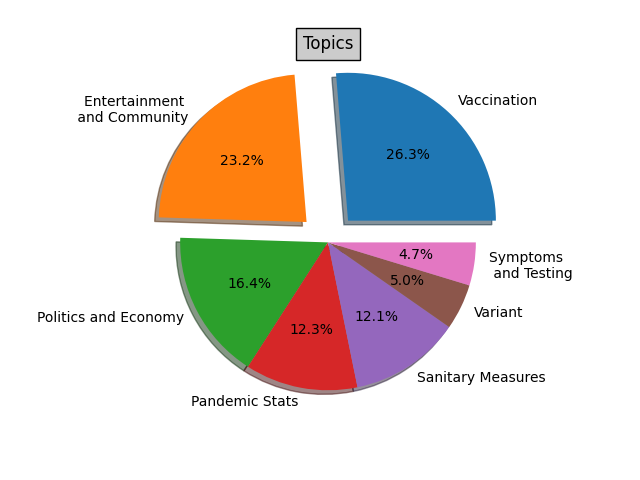
\includegraphics[width=0.9\columnwidth]{fig_topics} % Reduce the figure size so that it is slightly narrower than the column. Don't use precise values for figure width.This setup will avoid overfull boxes.
\caption{Topics split}.
\label{fig_topics}
\end{figure}

\begin{figure}[t]
\centering
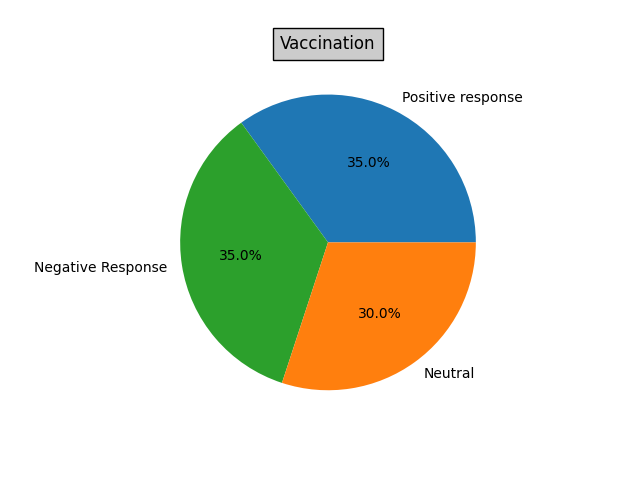
\includegraphics[width=0.9\columnwidth]{fig1} % Reduce the figure size so that it is slightly narrower than the column. Don't use precise values for figure width.This setup will avoid overfull boxes.
\caption{Most controversial topic}.
\label{fig_cont}
\end{figure}

% 1 page. Interpret your results in terms of what they reveal about the way each candidate was being discussed and perceived. Make extensive use of your results to justify your interpretations.

% Are insightful candidate-level interpretations provided? Are these grounded in results? Do the findings integrate results and prior knowledge in a sound, well-reasoned way?

Some topics had a much larger share of the total tweets than others. As seen in
Figure \ref{fig_topics}, the vaccination and entertainment and community were clear leaders in total tweets and almost represent half the tweets in the dataset with 49.5\% of the total share. This was to be expected as vaccination is the most controversial aspect of the COVID-19 pandemic and as social media users will use twitter to discuss the effects of the pandemic on their community and to discuss different aspects of the entertainment industry. 

Now three topics were in the middle of the pact: sanitary measures, politics and economy and pandemic. Sanitary measures and pandemic both represented 12.1\% and 12.3\% of the dataset respectively and politics and economy tweets represented 16.4\% of it. Thus, we can infer that these topics were relevant but not the most discussed at the time of the scraping. A reason behind this may be that these topics are more local than global. Indeed, these three topics characterize aspects of the COVID-19 pandemic that are more regional issues than global issues. A smaller subset of twitter users would then interact with them which consequently lowers their representation on the platform. 

Two topics were much less present in the dataset: variant and symptoms and testing. Both of these topics respectively represented less than or equal to 5\% of the dataset. These topics are thus clearly less prelevant on social media. In the case of the variant topic,  a major reason may be the very recent discovery of the Omicron variant and the containment of the Delta variant which may have lead to lesser representation of variants in the news and on social media. Consequently, due to the spontaenous and short nature of tweets, twitter users may have a smaller tendency to discuss them. In the case of the symptoms and testing topic, COVID-19 testing and symptoms are factual subjects that are extremely well documented online. Thus it is very easy to get access to information regarding them which may have lead to less people discussing them on social media.

Now the overall sentiment distribution of the tweets in the dataset is the following: 21.9\% negative, 50.6\% neutral and 27.5\% positive. This clearly shows that most tweets are factual, no matter the topic. A major reason behind this may be the short and concise nature of tweets which allows for information to be divulged to the large masses very rapidly. Consequently, tweets may often have been used to give updates on the current situation related to each one of the topics. 

For the vaccination topic, the distribution of the sentiment was very equal, as
seen in \ref{fig_cont}. Indeed, the proportion of tweets with negative sentiment is identical to the proportion of tweets with positive sentiment. Consequently, this gave an average sentiment of 0 which demonstrates that there were as many people for and against vaccination. The top words for this topic were all words related to vaccines, their efficacy, the companies creating them and regulating them. The word heart was also present. We can thus interpret that the discussions related to vaccination on Twitter were mainly about the efficacy of the vaccines and their side-effects such as heart diseases. 

The variant topic had an average sentiment of -0.1 which indicates a very slight negativity towards variants in twitter discussions. The top word for the topic is evidently omicron as this is most recent COVID-19 variant to emerge. Also, 3 words in the top 10 of topic 2 are directly related to South Korea. Thus, we can interpret that the discussions on twitter concerning variants have mostly been about the emergence of the Omicron variant in South Korea and the world. Combined with the slight negative average sentiment, we could interpret these discussions as fear towards a global spike in Omicron cases. 

On the other hand, the sanitary measures topic had an average sentiment of 0.09 which indicates a slight positivity towards the sanitary measures. The top 10 words with highest TF-IDF score are mostly related to the general restrictions put in place such as quarantine, restrictions, lockdowns. The presence of words such as passport and plane may indicate discussions related to COVID travel passports. Furthermore, combining the slight positivity indicated by the average sentiment with the top words, we can interpret that the discussions on twitter related to the sanitary measures may have been in slight favor of the restrictions put in place to slow down the spread of COVID-19.

Now the politics and economy topic had an average sentiment value of -0.037 which is negligible. The top 10 words with highest TF-IDF scores were all mostly related to American politics except for the words stocks and businesses. These two words combined with top words such as Trump, Biden, covid, senate hint that the discussions on twitter have been mainly about the handling of the covid epidemic in the United States and its effects on the economy. This may be due to the importance of the United States in the global economy and political landscape and also due to the fact that Twitter has a large part of its user base in the United States. 

The symptoms and testing topic had an average sentiment value of 0.085 which indicates a slight positive sentiment in the tweets related to symptoms and testing. The top words with highest TF-IDF score were related to possible remedies to the symptoms of COVID-19 such as the word vitamin and testing equipment such as swabs. The word margolin was also present which indicates the possibility of discussions about the new study lead by Dr. Leon Margolin on a possible over the counter COVID-19 treatment. The word myocarditis was also present which may indicate discussions about the long-term effects of COVID-19. In general, the overall neutral sentiment and top words for this topic indicate that discussions on Twitter revolved around the recovery steps of COVID-19 and side-effects after recovering from the virus.

Now the pandemic topic had an average sentiment value of 0.033 with is negligible. This does not come as a surprise as this topic mainly focused on facts and statistics which are two subject who mostly involve a neutral sentiment. The top 10 words for this topic varied a lot. Indeed, some words related to the progress of the pandemic such as normal, impact and averaging were present, but other words such as Orleans, visit, cruise and ship are also in the top 10. The presence of the words cruise, ship, Orleans seems to indicate possible discussions related to statistics related to the spread of COVID-19 on cruise ships which has been a controversial subject in the past year. Thus combining this assumption with the other words, we can interpret the discussions of the pandemic topic to mainly focus on statistics related to the most recent spread COVID-19 outbreaks.

Finally, the entertainment and community topic had a an average sentiment of 0.207 which is the largest average sentiment value within the topics. This positive average value is mostly due to the presence of tweets from fans encouraging their sports team or favorite musical artist. Indeed, this is shown in the top 10 words by TF-IDF score as the second most highest score goes to the word bts which is the name of a Korean band. Furthermore, after analyzing the dataset, most of the other words in the top 10 can be found in these tweets about BTS in which fans thank the band for entertaining them during the pandemic and wish them a happy vacation with their families. Also, word such as holidays and rest may be related to the start of the month of December and thus an indicator that twitter users are wishing each other happy holidays. Consequently, we can interpret the discussions about this topic to be mostly related to fans thanking their favorite musical artist, fans and people looking forward to the holidays.

Now our analysis is unfortunately not bulletproof. Indeed, a major weakness is the use of single annotation instead of double annotation. Unfortunately, due to time constraints, we were not able to perform double annotation which may lead to bias being present in our annotations. Another weakness is our inclusion of replies in our analysis. This could lead to major bias in the true underlying distribution of our topics in our dataset as some one our tweets may not be unique. Furthermore, this may be the exact reason why we have so many tweets about the Korean pop band BTS in our dataset. Our dataset size does not help reduce this bias either. This weakness is demonstrated by the top words by TF-IDF score for topic 7 being completely biased towards tweets involving BTS as the fans used similar language when tweeting.

Nevertheless, possible improvements we could integrate in the future to reduce these weaknesses could evidently be to use double annotation and also exclude replies from our parsing script. Furthermore, we could also gather a larger dataset which could help reduce the biases present in our data as the underlying distribution would converge to the true distribution according to the Law of Large Numbers. Finally, one aspect that would improve immensely that quality of this analysis is the use of deep learning algorithms. Indeed, we could train a simple bag of words model and transfer learning to then determine which key words would fit best for our query



% More data, better filtering (no replies etc.), wider variety of keywords

\section{Group Member Contributions}

The workload was distributed among the three team members. Their respective contributions are listed here: 

\  \textbf{Antoine Bonnet}: Wrote the data scraping for Twitter with Rahul and the script for computing TF-IDF scores for each category. Annotated a third of the data. Wrote the final report Data and Methods sections and computed statistics presented in the Results section.

\  \textbf{Rahul Kumar}: Wrote the data scraping for Twitter with Antoine.
Annotated a third of the data. Wrote a small portion of final report sections
(with Fabrizzio):  Introduction, Methods.

\  \textbf{Fabrizzio Sabelli}: Annotated a third of the data. Wrote the final report sections: Results, Discussion, Methods.
  
  
%\section{References}
\bibliography{refs}{}
\end{document}

